下のようなcountカウンターを書きます:


\begin{lstlisting}[numbers=none]
func count(w http.ResponseWriter, r *http.Request) {
    sess := globalSessions.SessionStart(w, r)
    ct := sess.Get("countnum")
    if ct == nil {
        sess.Set("countnum", 1)
    } else {
        sess.Set("countnum", (ct.(int) + 1))
    }
    t, _ := template.ParseFiles("count.gtpl")
    w.Header().Set("Content-Type", "text/html")
    t.Execute(w, sess.Get("countnum"))
}
\end{lstlisting}

count.gtplのコードは以下の通り:

\begin{lstlisting}[numbers=none]
Hi. Now count:{{.}}
\end{lstlisting}

ブラウザ上でリロードを行うと以下のような内容が確認できます:

\begin{figure}[H]
  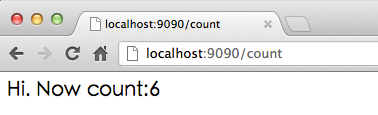
\includegraphics[width=8cm]{6.4.hijack.png}
   \label{図6.4}
   \caption{ブラウザでcount数を表示}
\end{figure}

リロードによって、数字は際限なく増加します。数字が6を示した時ブラウザ(ここではchromeを例にとります)のcookieマネージャを開くと、以下のような情報を見ることができます:

\begin{figure}[H]
  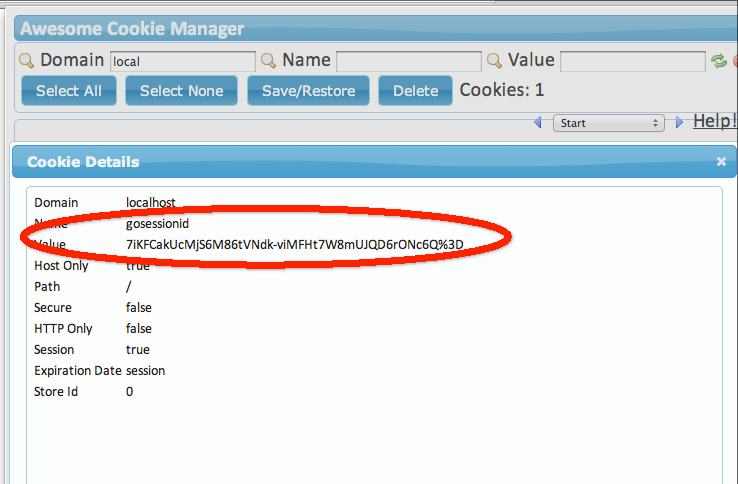
\includegraphics[width=14cm]{6.4.cookie.png}
   \label{図6.5}
   \caption{ブラウザが保存しているcookieを取得}
\end{figure}

次のステップが重要です:別のブラウザ(ここではfirefoxブラウザを開きました)を開き、chromeのアドレスバーのアドレスを新たに開いたブラウザのアドレスバーにコピーします。その後firefoxのcookieエミュレートプラグインを開き、新規にcookieを作成します。上の図のcookieの内容をそのままfirefoxの中に再設定します:

\begin{figure}[H]
  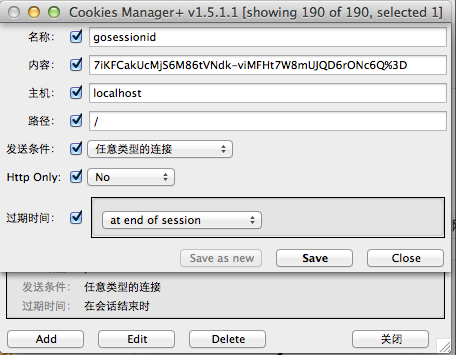
\includegraphics[width=8cm]{6.4.setcookie.png}
   \label{図6.6}
   \caption{cookieをエミュレート}
\end{figure}

エンターキーを押すと、下のような内容が現れます:

\begin{figure}[H]
  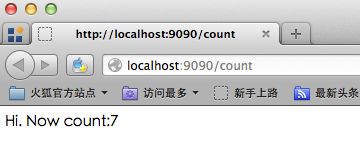
\includegraphics[width=8cm]{6.4.hijacksuccess.png}
   \label{図6.7}
   \caption{sessionのハイジャックに成功}
\end{figure}

ブラウザを変えても、sessionIDを取得することができました。この後cookieの保存過程をエミュレートします。この例は一台のコンピュータの上で行ったものです。たとえ二台によって行ったとしても結果は同じです。この時もし交代で2つのブラウザのリンクをクリックした場合、操作しているカウンターが実は同じものであるということに気づくでしょう。驚くことはありません。ここではfirefoxがchromeとgoserver間のセッション維持の鍵を盗みました。すなわち、gosessionidです。これは"セッションハイジャック"の一種です。goserverからすると、httpリクエストからgosessionidを得ました。HTTPプロトコルのステートレスによってgosessionidがchromeから"ハイジャック"されたものなんか知る方法はありません。依然として対応するsessionを探し、関連する計算を実行します。同時にchromeも自分が保持しているセッションがすでに"ハイジャック"されたことを知る方法もありません。

